%BEGIN TICKET 59
\begin{theorem}
    Пусть $f$ неотрицательная монотонная  $\!: [1, +\infty) \to \R$. Тогда:
     \[
    \left| \sum_{k=a}^b f(k) - \int\limits_a^b f(x)\mathrm{d}x \right| \le \max\{f(a), f(b)\} 
    .\] 
\end{theorem}
\begin{proof}
     $\sum\limits_{k=a}^{b-1} f(k) \ge \int\limits_a^b f(x)\mathrm{d}x \ge \sum\limits_{k=a+1}^b f(k)$. Не поняли? Рисуем картинку!
     \begin{figure}[!h]
         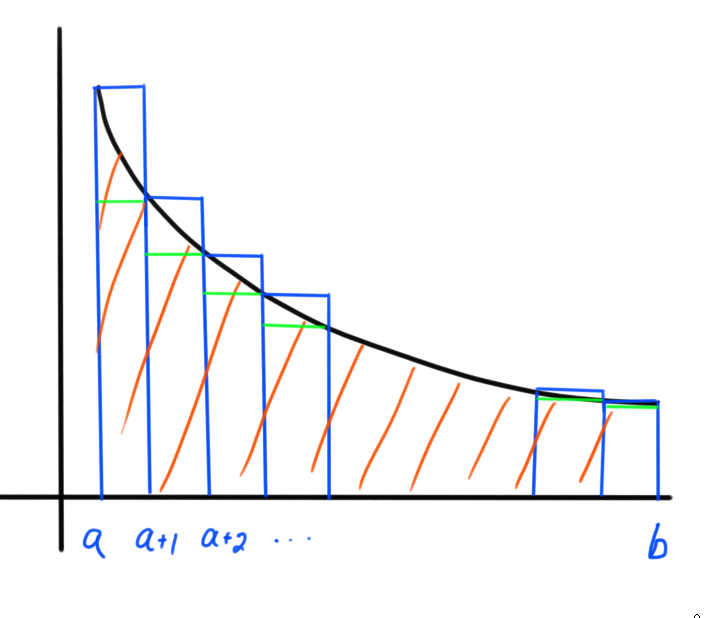
\includegraphics[scale=0.3]{integrals_and_sums}
     \end{figure}
    
    $\sum\limits_{k=a}^b f(k) - \int\limits_a^b \le \sum\limits_{k=a}^b - \sum\limits_{k=a-1}^b = f(a)$ (аналогично $f(b) = \sum\limits_{k=a}^b - \sum\limits_{k=a}^{b-1}$)

\end{proof}
\begin{theorem}[интегральный признак сходимости ряда]
    Пусть $f\!:[1, +\infty) \to \R$ неотрицательная, монотонно убывающая. 

    Тогда  $\sum\limits_{n=1}^\infty f(n)$ и  $\int\limits_1^\infty f(x) \mathrm{d}x$ ведут себя одинаково.
\end{theorem}
\begin{proof}
    По предыдущей теореме $S_n \coloneqq \sum\limits_{k=1}^n f(k) \ge \int\limits_1^n f(x)\mathrm{d}x \ge \sum\limits_{k=2}^n f(k) = S_n - f(1)$.

    Если ряд сходится, то $S_n$ --- ограничена  $\implies \int\limits_1^n f(x)\mathrm{d}x$ ограничена $\implies F(x) = \int\limits_1^x f$ --- ограничена $\implies \int\limits_1^\infty f(x)$ сходится.

    Если  $\int$ сходится $\implies \int\limits_1^n f$ --- ограничена  $\implies S_n$ --- ограничена  $\implies$ ряд сходится.
\end{proof}
\begin{example}
     \begin{enumerate}
         \item $\sum\limits_{n=1}^\infty \frac{1}{n^p}$, $p > 0$ (иначе члены ряда $\centernot \to 0$ и ряд расходится).\\
             $f(x) = \frac{1}{x^p}$. Монотонно убывает. $\sum \frac{1}{n^p}$ и $\int\limits_1^\infty \frac{\mathrm{d}x}{x^p}$ ведут себя одинаково: сходятся при  $p > 1$.
         \item $\sum\limits_{n=2}^\infty \frac{1}{n\ln n}$. $f(x) = \frac{1}{x\ln x}$ монотонно убывает. Поэтому $\int\limits_2^\infty \frac{\mathrm{d}x}{x\ln x}$ и $\sum\limits_{n=2}^\infty \frac{1}{n \ln n}$ ведут себя одинаково. 

             Там можно посчитать интеграл (разойдется).
    \end{enumerate}
\end{example}
\begin{consequence}
    \begin{enumerate}
        \item Если $a_n > 0$ и  $a_n = \mathcal{O}(\frac{1}{n^p})$ при $p > 1$ --- ряд  $\sum a_n$ --- сходится.
        \item Если  $a_n > 0$ и  $a_n \sim \frac{c}{n^p}$, то при $p > 1$ ряд  $\sum a_n$ --- сходится, а иначе расходится.
    \end{enumerate}
\end{consequence}
%END TICKET 59